\section*{Introduction}

Shapoid is a C library providing the \begin{ttfamily}Shapoid\end{ttfamily} structure and its functions which can be used to manipulate Shapoid objects (see next section for details).\\

It also provides the \begin{ttfamily}ShapoidIter\end{ttfamily} structure and its functions which can be used to sequantially loop through the surface/volume/... of a \begin{ttfamily}Shapoid\end{ttfamily}.\\

It uses the \begin{ttfamily}PBErr\end{ttfamily}, \begin{ttfamily}PBMath\end{ttfamily} and \begin{ttfamily}GSet\end{ttfamily} libraries.\\

\section{Definitions}

A Shapoid is a geometry defined by its dimension $D\in\mathbb{N^*_+}$ equals to the number of dimensions of the space it exists in, its position $\overrightarrow{P}$, and its axis $(\overrightarrow{A_0},\overrightarrow{A_1},...,\overrightarrow{A_{D-1}})$. $A_i$ and $P$ are vectors of dimension $D$. In what follows I'll use $I$ as notation for the interval $[0,D-1]$ for simplification.\\

Shapoids are classified in three groups: Facoid, Pyramidoid and Spheroid. The volume of a Shapoid is defined by, for a Facoid: 
\begin{equation}
\left\lbrace \sum_{i\in I}v_i\overrightarrow{A_i}+\overrightarrow{P}\right\rbrace ,v_i\in[0.0,1.0]
\end{equation}
for a Pyramidoid:
\begin{equation}
\left\lbrace \sum_{i\in I}v_i\overrightarrow{A_i}+\overrightarrow{P}\right\rbrace ,v_i\in[0.0,1.0], \sum_{i\in I}v_i\le1.0
\end{equation}
and for a Spheroid:
\begin{equation}
\begin{array}{rl}
\left\lbrace \sum_{i\in I}v_i\overrightarrow{A_i}+\overrightarrow{P}\right\rbrace ,&\\
v_i\in[-0.5,0.5],&\sum_{i\in I}v_i^2\le0.25
\end{array}
\end{equation}

\subsection{Transformation}

A translation of a Shapoid by $\overrightarrow{T}$ is obtained as follow:\\
\begin{equation}
\left(\overrightarrow{P},\left\lbrace\overrightarrow{A_i}\right\rbrace_{i\in I}\right)\mapsto\left(\overrightarrow{P}+\overrightarrow{T},\left\lbrace\overrightarrow{A_i}\right\rbrace_{i\in I}\right)
\end{equation} 
A scale of a Shapoid by $\overrightarrow{S}$ is obtained as follow:\\
\begin{equation}
\left(\overrightarrow{P},\left\lbrace\overrightarrow{A_i}\right\rbrace_{i\in I}\right)\mapsto\left( \overrightarrow{P},\left\lbrace\overrightarrow{A'_i}\right\rbrace_{i\in I}\right)
\end{equation} 
where
\begin{equation}
\overrightarrow{A'_i}=S_i\overrightarrow{A_i}
\end{equation}
For Shapoid whose dimension $D$ is equal to 2, a rotation by angle $\theta$ is obtained as follow:\\
\begin{equation}
\left(\overrightarrow{P},\overrightarrow{A_0},\overrightarrow{A_1}\right)\mapsto\left(\overrightarrow{P},\overrightarrow{A'_0},\overrightarrow{A'_1}\right)
\end{equation} 
where
\begin{equation}
\overrightarrow{A'_i}=\left[
\begin{array}{cc}
cos\theta&-sin\theta\\
sin\theta&cos\theta\\
\end{array}
\right]
\overrightarrow{A_i}
\end{equation}

\subsection{Shapoid's coordinate system}

The Shapoid's coordinate system is the system having $\overrightarrow{P}$ as origin and $\overrightarrow{A_i}$ as axis. One can change from the Shapoid's coordinate system ($\overrightarrow{X^S}$) to the standard coordinate system ($\overrightarrow{X}$) as follow:\\
\begin{equation}
\overrightarrow{X}=\left[\left(\overrightarrow{A_0}\right)\left(\overrightarrow{A_1}\right)...\left(\overrightarrow{A_{D-1}}\right)\right]\overrightarrow{X^S}+\overrightarrow{P}
\end{equation}
and reciprocally, from the standard coordinate system to the Shapoid's coordinate system:\\
\begin{equation}
\overrightarrow{X^S}=\left[\left(\overrightarrow{A_0}\right)\left(\overrightarrow{A_1}\right)...\left(\overrightarrow{A_{D-1}}\right)\right]^{-1}\left(\overrightarrow{X}-\overrightarrow{P}\right)
\end{equation}

\subsection{Insideness}

$\overrightarrow{X}$ is inside the Shapoid $S$ if, for a Facoid:\\
\begin{equation}
\forall i\in I,0.0\le X_i^S\le1.0
\end{equation}
for a Pyramidoid:\\
\begin{equation}
\left\lbrace\begin{array}{l}
\forall i\in I,0.0\le X_i^S\le1.0\\
\sum_{i\in I}X_i^S\le1.0
\end{array}\right.
\end{equation}
for a Spheroid:\\
\begin{equation}
\left|\left|\overrightarrow{X^S}\right|\right|\le0.5
\end{equation}

\subsection{Bounding box}

A bounding box of a Shapoid is a Facoid whose axis are colinear to axis of the standard coordinate system, and including the Shapoid in its volume. While the smallest possible bounding box can be easily obtained for Facoid and Pyramidoid, it's more complicate for Spheroid. Then we will consider for the Spheroid the bounding box of the equivalent Facoid $\left(\overrightarrow{P}-\sum_{i\in I}\left(0.5*\overrightarrow{A_i}\right),\left\lbrace\overrightarrow{A_i}\right\rbrace_{i\in I}\right)$ which gives the smallest bounding box when axis of the Spheroid are colinear to axis of the standard coordinate system and a bounding box slightly too large when not colinear.\\
The bounding box is defined as follow, for a Facoid:\\
\begin{equation}
\left(\overrightarrow{P'},\left\lbrace\overrightarrow{A'_i}\right\rbrace_{i\in I}\right)
\end{equation}
where\\
\begin{equation}
\left\lbrace
\begin{array}{l}
P'_i=P_i+\sum_{j\in I^-}A_{ji}\\
A'_{ij}=0.0,i\neq j\\
A'_{ij}=\sum_{k\in I^+}A_{kj}-\sum_{k\in I^-}A_{kj},i=j\\
\end{array}
\right.
\end{equation}
and, $I^+$ and $I^-$ are the subsets of $I$ such as $\forall j\in I^+,A_{ij}\ge 0.0$ and $\forall j\in I^-,A_{ij}<0.0$.\\

for a Pyramidoid:\\
\begin{equation}
\left(\overrightarrow{P'},\left\lbrace\overrightarrow{A'_i}\right\rbrace_{i\in I}\right)
\end{equation}
where\\
\begin{equation}
\left\lbrace
\begin{array}{l}
P'_i=P_i+Min\left(Min_{j\in I}(A_{ji}),0.0\right)\\
A'_{ij}=0.0,i\neq j\\
A'_{ij}=Max_{k\in I}(A_{kj})-Min_{k\in I}(A_{kj}),i=j\\
\end{array}
\right.
\end{equation}

\subsection{Depth and Center}

Depth $\mathbf{D}_S(\overrightarrow{X})$ of position $\overrightarrow{X}$ a Shapoid $S$ is a value ranging from 0.0 if $\overrightarrow{X}$ is on the surface of the Shapoid, to 1.0 if $\overrightarrow{X}$ is at the farthest location from the surface inside the Shapoid. Depth is by definition equal to 0.0 if $\overrightarrow{X}$ is outside the Shapoid. Depth is continuous and derivable on the volume of the Shapoid. It is defined by, for a Facoid:\\
\begin{equation}
\mathbf{D}_S(\overrightarrow{X})=\prod_{i\in I}\left(1.0-4.0*(0.5-X^S_i)^2\right)
\end{equation}
for a Pyramidoid:\\
\begin{equation}
\mathbf{D}_S(\overrightarrow{X})=\prod_{i\in I}\left(1.0-4.0*\left(0.5-\frac{X^S_i}{1.0-\sum_{j\in I-\lbrace i\rbrace}X^S_j}\right)^2\right)
\end{equation}
and for a Spheroid:\\
\begin{equation}
\mathbf{D}_S(\overrightarrow{X})=1.0-2.0*\left|\left|\overrightarrow{X^S}\right|\right|
\end{equation}
The maximum depth is obtained at $\overrightarrow{C}$ such as, for a Facoid:\\
\begin{equation}
\forall i\in I,C_i^S=0.5
\end{equation}
for a Pyramidoid:\\
\begin{equation}
\forall i\in I,C_i^S=\frac{1}{D+1}
\end{equation}
for a Spheroid:\\
\begin{equation}
\forall i\in I,C_i^S=0.0
\end{equation}
$\overrightarrow{C}$ is called the center of the Shapoid.

\subsection{Iterator on Spheroid}

While a sequential path through a Facoid and a Pyramidoid is obvious, path through a Spheroid is more complex. The solution implemented is described below.\\

Given a Spheroid of dimension $N$ we start from an arbitrary position: $<0,0,...,-0.5>$. From there we step the axis starting from the first one. If we could step an axis the step algorithm stops and return the new position as it could successfully step. However, if we could step on an axis other than the first one, it means we have modified the constraint for previous axis, the constraint being "is inside the spheroid". Then we reposition the axis before the stepped one to its lower possible value. It will allow it to step again at the next iteration on a new boundary defined by other axis values, and this scale up naturally to any dimension. Care must be care to the case when an axis reaches its upper value: the delta given by the user and the influence of other axis value make it jumps "over" the boundary in most cases. To keep things neat and clean we recalculate the exact value of the axis for its last step instead of using the delta given by the user.\\

The calculation of the lower and upper values of an axis given the values of other axis can be performed as follow:\\

Lets note $\overrightarrow{P}=<p_0,p_1,...,p_{N-1}>$ the position in a Spheroid of dimension $N$. A position will be on the boundary of the Spheroid if and only if $||\overrightarrow{P}||=0.5$. We want to calculate $\alpha$ which bring a position $\overrightarrow{P'}$ inside the Spheroid to a position $\overrightarrow{P}$ on the boundary of the Spheroid by modifying the axis $i$ (i.e. $p_i=p'_i+\alpha$ and $p_j=p'_j,j\neq i$). Lets note $n=||\overrightarrow{P'}||$. We have:\\

\begin{equation}
\label{eqWormyA}
p'^2_0+p'^2_1+...+p'^2_i+...+p'^2_{N-1}=n^2
\end{equation}
and \\
\begin{equation}
p^2_0+p^2_1+...+p^2_i+...+p^2_{N-1}=0.25
\end{equation}
equivalent to \\
\begin{equation}
\label{eqWormyB}
p'^2_0+p'^2_1+...+(p'_i+\alpha)^2+...+p'^2_{N-1}=0.25
\end{equation}
by substracting \eqref{eqWormyA} and \eqref{eqWormyB} we have\\
\begin{equation}
p'^2_i-(p'_i+\alpha)^2=n^2-0.25
\end{equation}
equivalent to\\
\begin{equation}
p'^2_i-(p'^2_i+\alpha^2+2p'_i\alpha)=n^2-0.25
\end{equation}
equivalent to\\
\begin{equation}
-\alpha^2-2p'_i\alpha-(n^2-0.25)=0
\end{equation}
simplified to\\
\begin{equation}
\alpha^2+2p'_i\alpha+(n^2-0.25)=0
\end{equation}
This quadratic equation can be solved directly to obtain $\alpha$:\\
\begin{equation}
\alpha=\frac{-2p'_i\pm\sqrt{4p'^2_i-4(n^2-0.25)}}{2}
\end{equation}
Which gives the two solutions defining the lower and upper boundaries of the Spheroid on the axis $i$.\\

This result can then be used to solve our problem with what I'll call the "Wormy Algorithm":\\

\begin{scriptsize}
\begin{ttfamily}
\verbatiminput{/home/bayashi/GitHub/Shapoid/wormy.txt}
\end{ttfamily}
\end{scriptsize}

This algorithm step $P$ to the next position in the path by $delta$ and returns true if we haven't reached the end of the path, or false if we have reached the end of the path (i.e. if we have iterated through all the surface/volume/... of the Spheroid). Remember that $P$ must be initialised to $<0,0,...,-0.5>$ as the beginning of the path, and that \begin{ttfamily}ShapoidIter\end{ttfamily} iterates coordinates in the Shapoid's coordinate system.\\

\subsection{Collision detection of Spheroid}

The detection of collision between two Spheroids is done as follow. One of the spheroid is converted into the coordinates system of the other and checked against a circle of radius 0.5 centered at the origin of the system. By checking that the position of the converted Spheroid is less than its minor radius plus 0.5 or more than its major radius plus 0.5, the trivial cases of, respectively, interesection and non intersection can be performed. In other cases an incremental search from the center of the converted Spheroid toward the nearest point to the origin inside this Spheroid is performed. The intersection can then be checked by testing if the distance of this point to the origin is less or equal than 0.5.\\

\subsection{Collision detection between Facoid and Pyramidoid}

The intersection detection is impletemented for 2D and 3D static cases only. For optimal performance, in 2D the SAT algorithm is used, in 3D the FMB algorithm is used.

\section{Interface}

\begin{scriptsize}
\begin{ttfamily}
\verbatiminput{/home/bayashi/GitHub/Shapoid/shapoid.h}
\end{ttfamily}
\end{scriptsize}

\section{Code}

\subsection{shapoid.c}

\begin{scriptsize}
\begin{ttfamily}
\verbatiminput{/home/bayashi/GitHub/Shapoid/shapoid.c}
\end{ttfamily}
\end{scriptsize}

\subsection{shapoid-inline.c}

\begin{scriptsize}
\begin{ttfamily}
\verbatiminput{/home/bayashi/GitHub/Shapoid/shapoid-inline.c}
\end{ttfamily}
\end{scriptsize}

\section{Makefile}

\begin{scriptsize}
\begin{ttfamily}
\verbatiminput{/home/bayashi/GitHub/Shapoid/Makefile}
\end{ttfamily}
\end{scriptsize}

\section{Unit tests}

\begin{scriptsize}
\begin{ttfamily}
\verbatiminput{/home/bayashi/GitHub/Shapoid/main.c}
\end{ttfamily}
\end{scriptsize}

\section{Unit tests output}

\begin{scriptsize}
\begin{ttfamily}
\verbatiminput{/home/bayashi/GitHub/Shapoid/unitTestRef.txt}
\end{ttfamily}
\end{scriptsize}

facoid.txt

\begin{scriptsize}
\begin{ttfamily}
\verbatiminput{/home/bayashi/GitHub/Shapoid/facoid.txt}
\end{ttfamily}
\end{scriptsize}

Example of path on a 2D Spheroid using the ShapoidIterator:\\

\begin{center}
\begin{figure}[H]
\centering
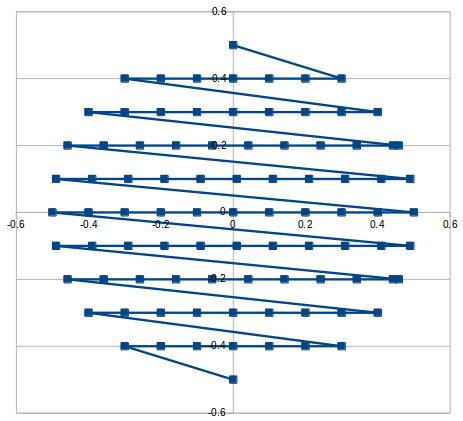
\includegraphics[width=12cm]{./spheroid2dpath.png}
\end{figure}
\end{center}
